%-------------------------
% One-Page Modern Resume in LaTeX
% Author : Md. Arafatuzzaman
% Optimized single-page layout
%------------------------

\documentclass[letterpaper,11pt]{article}

\usepackage{latexsym}
\usepackage[empty]{fullpage}
\usepackage{titlesec}
\usepackage{marvosym}
\usepackage[usenames,dvipsnames]{color}
\usepackage{verbatim}
\usepackage{enumitem}
\usepackage[hidelinks]{hyperref}
\usepackage{fancyhdr}
\usepackage[english]{babel}
\usepackage{tabularx}
\usepackage{fontawesome5}
\usepackage{multicol}
\usepackage[T1]{fontenc}
\usepackage{helvet}
\usepackage{graphicx}
\usepackage{tikz}
\usepackage{xcolor}
\usetikzlibrary{shadows.blur,positioning}

\renewcommand{\familydefault}{\sfdefault}
\setlength{\multicolsep}{-3.0pt}
\setlength{\columnsep}{-1pt}
\input{glyphtounicode}

% Elegant color scheme
\definecolor{headerDark}{RGB}{25, 42, 86}
\definecolor{primaryBlue}{RGB}{52, 109, 219}
\definecolor{accentGold}{RGB}{255, 193, 7}
\definecolor{darkText}{RGB}{33, 37, 41}
\definecolor{mediumGray}{RGB}{108, 117, 125}

\pagestyle{fancy}
\fancyhf{}
\fancyfoot{}
\renewcommand{\headrulewidth}{0pt}
\renewcommand{\footrulewidth}{0pt}

% Optimized margins for one page
\addtolength{\oddsidemargin}{-0.65in}
\addtolength{\evensidemargin}{-0.65in}
\addtolength{\textwidth}{1.3in}
\addtolength{\topmargin}{-.85in}
\addtolength{\textheight}{1.6in}

\urlstyle{same}
\raggedbottom
\raggedright
\setlength{\tabcolsep}{0in}

% Compact section formatting
\titleformat{\section}{
  \vspace{-6pt}\raggedright\large\bfseries\color{headerDark}
}{}{0em}{}[\color{primaryBlue}\titlerule\vspace{-4pt}]

\pdfgentounicode=1

% Compact custom commands
\newcommand{\resumeItem}[1]{
  \item\small{#1 \vspace{-1pt}}
}

\newcommand{\resumeSubheading}[4]{
  \vspace{-1pt}\item
    \begin{tabular*}{1.0\textwidth}[t]{l@{\extracolsep{\fill}}r}
      \textbf{\color{darkText}#1} & \textbf{\small\color{primaryBlue} #2} \\
      \textit{\small\color{mediumGray}#3} & \textit{\small\color{mediumGray} #4} \\
    \end{tabular*}\vspace{-5pt}
}

\newcommand{\resumeProjectHeading}[2]{
    \vspace{-1pt}\item
    \begin{tabular*}{1.0\textwidth}{l@{\extracolsep{\fill}}r}
      \small\textbf{\color{darkText}#1} & \textbf{\small\color{primaryBlue} #2}\\
    \end{tabular*}\vspace{-5pt}
}

\renewcommand\labelitemi{$\vcenter{\hbox{\tiny$\bullet$}}$}

\newcommand{\resumeSubHeadingListStart}{\begin{itemize}[leftmargin=0.0in, label={}]}
\newcommand{\resumeSubHeadingListEnd}{\end{itemize}}
\newcommand{\resumeItemListStart}{\begin{itemize}[leftmargin=0.15in]}
\newcommand{\resumeItemListEnd}{\end{itemize}\vspace{-3pt}}

%-------------------------------------------
%%%%%%  RESUME STARTS HERE  %%%%%%%%%%%%%%%%%%%%%%%%%%%%

\begin{document}

%----------COMPACT HEADER----------
\begin{tikzpicture}[remember picture,overlay]
    % Dark header background
    \fill[headerDark] (current page.north west) rectangle ([yshift=-3.2cm]current page.north east);
    % Accent line
    \fill[accentGold] ([yshift=-3.2cm]current page.north west) rectangle ([yshift=-3.3cm]current page.north east);
    % Decorative elements
    \fill[primaryBlue,opacity=0.1] ([xshift=-2cm,yshift=-0.8cm]current page.north east) circle (2.5cm);
    \fill[accentGold,opacity=0.08] ([xshift=2cm,yshift=-2.5cm]current page.north west) circle (2cm);
\end{tikzpicture}

\vspace{12pt}

\begin{center}
    % Compact profile photo
    \begin{tikzpicture}
        \fill[black!20] (0.06,-0.06) circle (1.1cm);
        \fill[white] (0,0) circle (1.08cm);
        \begin{scope}
            \clip (0,0) circle (0.95cm);
            \node at (0,0) {\includegraphics[width=1.9cm]{profile.jpg}};
        \end{scope}
        \draw[line width=2pt, accentGold] (0,0) circle (1.03cm);
    \end{tikzpicture}
    
    \vspace{6pt}
\end{center}

% Compact name section
\vspace{-12pt}
\begin{center}
    {\LARGE\bfseries\color{headerDark} MD. ARAFATUZZAMAN} \\ 
    \vspace{3pt}
    {\normalsize\color{primaryBlue}\textit{Developer | IoT Enthusiast | AI/ML Explorer}} \\ 
    \vspace{8pt}
    
    % Compact contact info
    \begin{tikzpicture}
        \fill[white,rounded corners=6pt] (-7,-0.65) rectangle (7,0.65);
        \node[align=center] at (0,0) {
            \footnotesize
            \begin{tabular}{c@{\hspace{1cm}}c@{\hspace{1cm}}c@{\hspace{1cm}}c}
                \textcolor{primaryBlue}{\large\faIcon{phone}} & 
                \textcolor{primaryBlue}{\large\faIcon{envelope}} & 
                \textcolor{primaryBlue}{\large\faIcon{linkedin}} & 
                \textcolor{primaryBlue}{\large\faIcon{github}} \\[3pt]
                \href{tel:+8801522100079}{\color{darkText}\textbf{+8801522100079}} & 
                \href{mailto:makky.cse@gmail.com}{\color{darkText}\textbf{makky.cse@gmail.com}} & 
                \href{https://linkedin.com/in/md-amakky}{\color{darkText}\textbf{md-amakky}} & 
                \href{https://github.com/mdmakky}{\color{darkText}\textbf{mdmakky}}
            \end{tabular}
        };
    \end{tikzpicture}
    \vspace{4pt}
\end{center}

%-----------SUMMARY-----------
\section{\texorpdfstring{\faIcon{user}\ }{User }Professional Summary}
\small{\color{darkText}Computer Science graduate specializing in full-stack development with React, FastAPI, and Python. Experienced in IoT systems, AI/ML integration with RAG architectures, and building collaborative web platforms. Proven ability to develop responsive UIs, robust APIs, and intelligent document analysis systems.}
\vspace{-4pt}

%-----------EDUCATION-----------
\section{\faIcon{graduation-cap}\ Education}
  \resumeSubHeadingListStart
    \resumeSubheading
      {Jashore University of Science and Technology}{Graduated: 2024}
      {Bachelor of Science in Computer Science \& Engineering}{CGPA: 3.17/4.0}
  \resumeSubHeadingListEnd
\vspace{-6pt}

%-----------TECHNICAL SKILLS-----------
\section{\faIcon{code}\ Technical Skills}
 \begin{itemize}[leftmargin=0.15in, label={}]
    \small{\item{
     \textbf{\color{headerDark}Frontend:} \color{darkText}React.js, JavaScript (ES6+), HTML5, CSS3, TailwindCSS \\
     \textbf{\color{headerDark}Backend:} \color{darkText}FastAPI, Python, Node.js, Express.js, REST APIs \\
     \textbf{\color{headerDark}Databases:} \color{darkText}PostgreSQL, SQLite, MongoDB, ChromaDB (Vector DB)\\
     \textbf{\color{headerDark}IoT \& Hardware:} \color{darkText}Raspberry Pi, Python GPIO, Computer Vision, Sensor Integration\\
     \textbf{\color{headerDark}AI/ML:} \color{darkText}Langchain, Google Gemini AI, RAG Systems, PyTorch, NLP \\
     \textbf{\color{headerDark}Tools:} \color{darkText}Git, GitHub, Vite, Linux, Docker, Chrome Extensions
    }}
 \end{itemize}
 \vspace{-8pt}

%-----------PROJECTS-----------
\section{\faIcon{laptop-code}\ Projects}
    \resumeSubHeadingListStart
    
      \resumeProjectHeading
          {\textbf{PetNest (Team Project)} $|$ \emph{\color{mediumGray}JavaScript, Node.js, Express, MongoDB, React}}{\href{https://github.com/mdmakky/PetNest}{GitHub}}
          \resumeItemListStart
            \resumeItem{\color{darkText}Created full-featured pet adoption platform with RESTful APIs for authentication, listings, and services}
            \resumeItem{\color{darkText}Built responsive React frontend with search, filter features and MongoDB database schema}
          \resumeItemListEnd
          
      \resumeProjectHeading
          {\textbf{Mentora AI} $|$ \emph{\color{mediumGray}React, FastAPI, Python, Langchain, Google Gemini AI}}{\href{https://github.com/mdmakky/Mentora}{GitHub}}
          \resumeItemListStart
            \resumeItem{\color{darkText}AI-powered PDF study assistant with RAG system for document-specific Q\&A and analytics dashboard}
            \resumeItem{\color{darkText}Built with React frontend, FastAPI backend, ChromaDB vector storage for intelligent document analysis}
          \resumeItemListEnd
          
      \resumeProjectHeading
          {\textbf{Share-Reads WebAPP (Team Project)} $|$ \emph{\color{mediumGray}EJS, Node.js, Express, MongoDB}}{\href{https://github.com/mdmakky/Share-Reads-WebAPP}{GitHub}}
          \resumeItemListStart
            \resumeItem{\color{darkText}Book sharing platform with user profiles, reviews, ratings, and server-side rendering using EJS}
          \resumeItemListEnd
          
      \resumeProjectHeading
          {\textbf{Facebook Element Hider} $|$ \emph{\color{mediumGray}JavaScript, Chrome Extension, DOM Manipulation}}{\href{https://github.com/mdmakky/Facebook-Cleaner}{GitHub}}
          \resumeItemListStart
            \resumeItem{\color{darkText}Chrome extension for customizable Facebook UI cleanup with instant CSS hiding and smart element detection}
          \resumeItemListEnd
    
    \resumeSubHeadingListEnd
\vspace{-6pt}

%-----------ACHIEVEMENTS-----------
\section{\faIcon{trophy}\ Achievements \& Activities}
 \begin{itemize}[leftmargin=0.15in, label={}]
    \small{\item{
     \textbf{\color{headerDark}Competitive Programming:} \color{darkText}Participated in CTF competitions and cybersecurity challenges \\
     \textbf{\color{headerDark}Hackathons:} \color{darkText}Active participant collaborating on innovative solutions under time constraints \\
     \textbf{\color{headerDark}Robosociety Member:} \color{darkText}University robotics society, working on IoT and hardware projects \\
     \textbf{\color{headerDark}Open Source:} \color{darkText}Active GitHub contributor with multiple public repositories
    }}
 \end{itemize}
 \vspace{-8pt}

%-----------CERTIFICATIONS-----------
\section{\faIcon{certificate}\ Certifications}
    \resumeSubHeadingListStart
      \resumeProjectHeading
          {\textbf{Digital Skills 4 Students - AI/ML Course}}{Bangladesh Govt Initiative}
      \resumeProjectHeading
          {\textbf{Member - Robosociety}}{JUST}
    \resumeSubHeadingListEnd

\end{document}